%%%%%%%%%%%%%%%%%%%%%%%%%%%%%%%%%%%%%%%%%%%%%%%%%%%%%%%%%%%%%%%%%%%%%%%%%%%%
%% Conference version (complete paper, 10-page limit).
%% Formatting per workshop requirements:
%%   - 12-point font, one-inch margins on all four sides, US letter (8.5 x 11).
%%   - Blinded (no author/affiliation information).
%%   - No copyright-ownership notice is included.
%% Compile in the same project as the journal source: it reuses refs.bib,
%% informs2014.bst, and the figure directories (Figures/, Rebuttal-R1/).
%%%%%%%%%%%%%%%%%%%%%%%%%%%%%%%%%%%%%%%%%%%%%%%%%%%%%%%%%%%%%%%%%%%%%%%%%%%%
\documentclass[12pt,letterpaper]{article}
\usepackage[margin=1in]{geometry}

\usepackage{amsmath}
\usepackage{newtxtext,newtxmath}   % provides AMS symbols; do NOT also load amssymb
\usepackage{mathtools,bm}
\usepackage{dsfont}                % \mathds{1} for the indicator
\usepackage{graphicx}
\usepackage{booktabs}
\usepackage{multirow}
\usepackage{array}
\usepackage{caption}
\usepackage{subcaption}
\usepackage{xcolor}

\usepackage{natbib}
\bibpunct[, ]{(}{)}{,}{a}{}{,}%
\def\bibfont{\fontsize{9}{10.5}\selectfont}%  % 9pt references to fit the page budget
\def\bibsep{1pt plus 0.3pt}%
\def\bibhang{16pt}%
\def\newblock{\ }%
\def\BIBand{and}%   % required by the INFORMS informs2014.bst

\usepackage[colorlinks=true,allcolors=blue]{hyperref}

% ---- spacing tuned for the page budget ----
\captionsetup{font=small,labelfont=bf,skip=4pt}
\linespread{0.96}          % slight global leading reduction (tighter, no line overlap)
\setlength{\parskip}{0pt}
\setlength{\textfloatsep}{9pt plus 2pt minus 2pt}
\setlength{\intextsep}{9pt plus 2pt minus 2pt}
\setlength{\floatsep}{9pt plus 2pt minus 2pt}
% let pages hold more float+text so figures don't leave half-empty pages
\renewcommand{\topfraction}{0.92}
\renewcommand{\bottomfraction}{0.9}
\renewcommand{\textfraction}{0.06}
\renewcommand{\floatpagefraction}{0.85}

% ---- macros ----
\newcommand{\bx}{\mathbf{x}}
\newcommand{\bX}{\mathbf{X}}
\newcommand{\mD}{\mathcal{D}}
\newcommand{\mG}{\mathcal{G}}
\newcommand{\mM}{\mathcal{M}}
\newcommand{\mE}{\mathcal{E}}
\newcommand{\Xto}{\mathbf{X}\mapsto Y}
\newcommand{\Xtohat}{\mathbf{X}\mapsto \hat{Y}}

\title{\bf From Model Explanation to Data Misinterpretation:\\
A Cautionary Analysis of Post Hoc Explainers in Business Research}

% ---- BLINDED: no author or affiliation information ----
\author{}
\date{}

\begin{document}
\maketitle

\begin{abstract}
\noindent
Post hoc explainers such as SHAP and LIME are widely used in business research to
interpret complex machine learning (ML) models. Although they were designed to
explain a \emph{model}'s decision-making process---the mapping from $\bX$ to
$\hat{Y}$---a growing body of work treats the explanations
they produce as evidence about underlying variable relationships in the data. Based on a
systematic review of 181 studies, including 56 published in leading journals, we
document that this practice is widespread and examine its validity. We introduce
two metrics---\emph{direction alignment} and \emph{strength alignment}---and use
simulated data with known ground truth to assess how well SHAP and LIME recover
the direction and relative importance of features in the true data-generating
process. Although explanations often appear reasonable \emph{on average}, they
exhibit substantial heterogeneity, with long-tailed failures that persist even
when predictive accuracy is high: high accuracy is \emph{necessary but
insufficient} for reliable explanation. We show that feature correlation and the
\emph{Rashomon effect}---many equally accurate models relying on different
decision-making processes---are the key drivers of misalignment, and that \emph{agreement in
explanations} across such models provides a practical, dataset-level diagnostic
of reliability. Our findings caution against using post hoc explainers to
\emph{validate} hypotheses and instead position them as exploratory tools that
\emph{generate}, rather than confirm, substantive insights.

\smallskip
\noindent\textbf{Keywords:} post hoc explanation; interpretable machine learning;
SHAP; LIME; Rashomon set; research methodology.
\end{abstract}

%======================================================================
\section{Introduction}
\label{sec:intro}

The growth in data volume and complexity has made machine learning (ML) a mainstay
of business analytics, particularly for prediction \citep{kleinberg2015prediction,
mullainathan17applied}. Yet prediction alone is rarely the goal. Researchers and
managers also want to understand their data---in particular, \emph{how explanatory
variables ($\bX$) relate to an outcome ($Y$)}: for instance, which product attributes drive customer satisfaction, how price and promotion affect demand, or which borrower characteristics raise default risk. Because most high-accuracy ML models
are black boxes, \emph{post hoc explainers} have become the standard tool
for peering inside them. For example, SHAP (SHapley Additive
exPlanations) \citep{lundberg17shap} assigns each feature a Shapley value
representing its contribution to a prediction relative to a baseline, while LIME
(Local Interpretable Model-agnostic Explanations) \citep{ribeiro16lime} fits
a sparse local linear surrogate around an instance. Both report the direction and
strength with which features influence a model's predictions.

A growing body of empirical business research adopts these explainers through a
two-stage \emph{explanation pipeline} (Figure~\ref{fig:pipeline}):
a black-box model is trained for a prediction task, and a post hoc explainer is then
applied to it. Used as intended, this pipeline illuminates \emph{model} behavior---which
features the model relies on. Increasingly, however, business researchers reinterpret the
same output as evidence about the \emph{data}: they generalize explanations of the
model's mapping ($\Xtohat$), which are inherently model-dependent, into claims about
the true relationship in the data ($\Xto$). For example, \citet{park2024extracting}
read SHAP values as which smartphone features customers prefer; \citet{jiang24churn}
treat features with large SHAP values as churn drivers; and
\citet{sanchez2023role} use SHAP to identify drivers of hotel-guest satisfaction and
motivate managerial action. Some work even proposes ML-plus-SHAP as an ``alternative
to OLS'' \citep{berger2023supply}.

\begin{figure}[t]
\centering
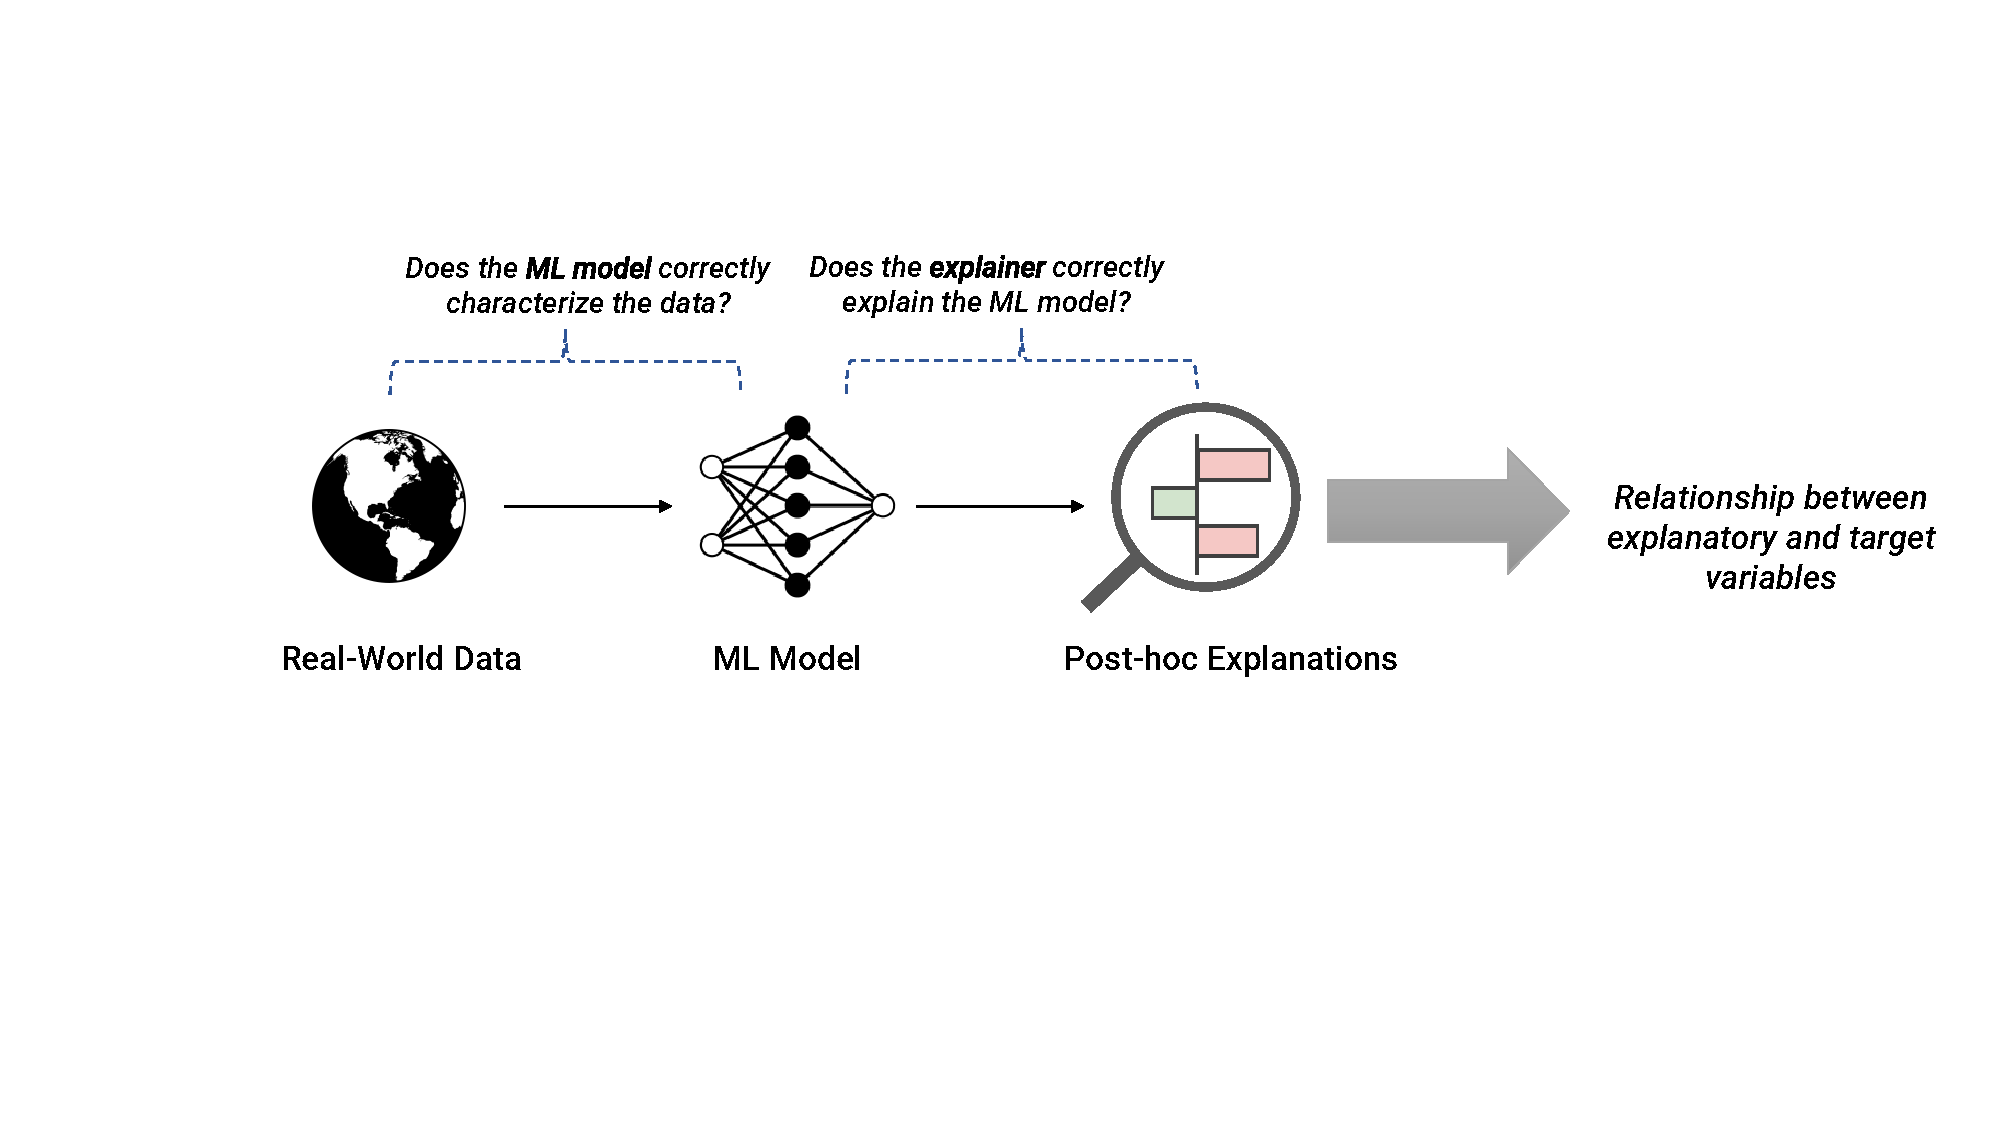
\includegraphics[trim={4.75cm 7.5cm 1.125cm 4.25cm},clip,width=0.95\textwidth]{Figures/pipeline_flow_new.pdf}
\caption{The explanation pipeline. A black-box model is trained for prediction and
then explained by a post hoc explainer. Inferring the true marginal effects of
features from these explanations---the step marked in red---constitutes a mistaken
use of the pipeline.}
\label{fig:pipeline}
\end{figure}

To gauge prevalence, we manually reviewed 181 papers that make substantive
use of SHAP or LIME. Roughly \textbf{42.5\%} interpret post hoc explanations as
evidence of \emph{data-level} relationships rather than statements about the
model---indicating that the practice is widespread in business research; the rate
is lower but still nontrivial in leading journals (16.1\% in \textit{UTD~24},
\textit{FT50}, and INFORMS).

We stress that this is a \emph{new} question, and one that is distinctively a
concern for business research. Post hoc explainers have been scrutinized
extensively in computer science, but that work asks whether an explanation
faithfully describes the \emph{model}---the mapping $\Xtohat$ it was applied to.
Business research asks something that literature does not: whether the same
explanation can be read as evidence about the \emph{data}, the mapping $\Xto$ in
the world. The two are routinely conflated yet logically distinct, and the validity
of the data-level reading---the inference our review shows empirical studies
actually draw, and which drives managerial conclusions---has never been
systematically tested. This motivates our central question:
\begin{quote}
\emph{To what extent can explanations derived from a machine learning model
($\Xtohat$) recover the direction and relative strength of the true relationship
in the data ($\Xto$)?}
\end{quote}

Our study proceeds in four steps. \textbf{First}, we formalize the two claims that
prior business studies using post hoc explanations implicitly rely on. \emph{Direction} interpretations assert that
increasing a feature increases or decreases the outcome; \emph{strength}
interpretations rank features by importance. We give method-agnostic definitions of
\emph{direction alignment} and \emph{strength alignment} that apply to any explainer
that assigns a value to each feature. \textbf{Second}, we evaluate SHAP and LIME on simulated data where the
ground-truth $\Xto$ is known and precisely controlled. Although explanations look
truthful on average, their alignment with the ground truth is highly heterogeneous, with pronounced
long-tailed deviations---even when the black-box model's predictive accuracy is high---so that a
researcher typically cannot tell \emph{when} an explanation is trustworthy.
\textbf{Third}, we trace the drivers of misalignment to (i) the predictive
performance of the model, (ii) the \emph{Rashomon effect}
\citep{semenova22rashomon,paes23inevitable}, and (iii) data properties such as
feature correlation. The central lesson is that high accuracy is \emph{necessary
but insufficient}: equally accurate models can rely on markedly different
decision-making processes, thus yielding different
explanations, and feature correlation is the dominant data-level driver of
disagreement. \textbf{Fourth}, we show that \emph{disagreement among equally
accurate models} is a usable diagnostic. Agreement based on \emph{explanations}
 is strongly correlated with alignment, whereas prediction-based agreement is not. Rashomon
agreement thus provides a practical, dataset-level signal of when explanations of
$\Xtohat$ are unlikely to recover $\Xto$.

Overall, we caution against a growing trend of using post hoc explanations to draw
inferences about data. Explanations should not be used to \textbf{validate}
hypotheses about $\Xto$; their proper role is to \textbf{propose} hypotheses that
are then tested with methods built for identification---as a growing number of
studies already do \citep{zhang2023can,feng2025ai,senoner2022using}. Keeping exploration and
validation distinct avoids overstating the reliability of
explainer-derived insights.

The rest of the paper is organized as follows.
Section~\ref{sec:related} reviews SHAP, LIME, and the Rashomon effect.
Section~\ref{sec:metrics} defines the data-level claims we test and our alignment
metrics and simulation design.
Section~\ref{sec:results} reports whether explanations align with the data and
checks the result's robustness;
Section~\ref{sec:factors} isolates the drivers of misalignment.
Section~\ref{sec:diag} develops the Rashomon-agreement diagnostic, and
Section~\ref{sec:concl} concludes with guidance for practice.

%======================================================================
\section{Background and Related Work}
\label{sec:related}

\vspace{-3mm}
\paragraph{SHAP and LIME.}
SHAP \citep{lundberg17shap} attributes a prediction to features using the Shapley
value from cooperative game theory. Its appeal rests on two properties:
\emph{local accuracy} (feature contributions sum to the prediction minus its
baseline) and \emph{consistency} (making a feature more important cannot decrease
its attribution). LIME \citep{ribeiro16lime} perturbs an instance, weights the
perturbations by proximity, and fits a sparse linear surrogate whose coefficients
are read as local feature influences. Both are model-agnostic and report a
direction (sign) and a strength (magnitude) per feature; global importance is
usually taken to be the mean absolute attribution across instances.

\vspace{-3mm}
\paragraph{Scrutiny in computer science.}
The ML literature has scrutinized both methods extensively, but at the \emph{model}
level---whether an explanation faithfully describes the fitted model: LIME is
unstable across sampling and kernel choices
\citep{garreau2020looking,alvarez18robustness}, explanations can be adversarially
manipulated \citep{slack19fooling}, and Shapley-value attributions have been
criticized as ill-suited to human notions of importance \citep{kumar20shap,han22which}.
Notably, even the sharpest of these critiques concern specific failure
contexts---models deliberately engineered to deceive the explainer
\citep{slack19fooling}, or counterfactual decision tasks the tools were not
designed for \citep{fernandez20explaining}---and none tests whether an explanation
applied in good faith to a well-trained model recovers relationships in the
\emph{data}.
Model-level faithfulness, even where it holds, does not imply data-level validity.

\vspace{-3mm}
\paragraph{Engagement in business and management.}
The business and management community has engaged with these tools just as
actively, but from an applied, consequential angle. One stream studies how
explainable AI shapes managerial and user decision-making \citep{bauer23infoproc,
von2025knowing}, including in high-stakes domains such as healthcare
\citep{hassan25unlocking} and misinformation detection \citep{lee24false}, and the
regulatory and compliance challenges it raises---especially in credit scoring
\citep{mohammadi2025regulating,bucker2022transparency,chen2024interpretable}. A
parallel methodological stream advances new or improved explanations, for instance
contrasting feature attributions with counterfactuals \citep{fernandez20explaining}
or refining LIME's sampling and surrogate-fitting stages \citep{kim2023rolex}.
This body of work has meaningfully advanced how the field deploys and governs post
hoc explainers.


\vspace{-3mm}
\paragraph{Where our question sits.}
Crucially, both literatures evaluate explanations \emph{of the model} ($\Xtohat$)---
whether they faithfully or usefully describe the fitted predictor. Our question is
one step further removed and, for empirical research, more consequential: whether
explanations of $\Xtohat$ license conclusions about the data itself ($\Xto$). This
is the very inference that econometric tools---regression, causal inference,
experiments---are built to support by making identification assumptions explicit,
whereas post hoc explainers were designed only to describe a fitted model.

\vspace{-3mm}
\paragraph{The Rashomon effect.}
For a given task there is often a \emph{Rashomon set}: many models with nearly
identical predictive performance but different internal structure and feature
attributions \citep{semenova22rashomon,paes23inevitable,rudin2024amazingthingscomehaving}.
Each such model encodes a distinct hypothesis about $\Xto$. Consequently, even a
perfect explanation of a \emph{single} model need not reflect the true relationship
in the data---a point that motivates both our misalignment analysis and our
diagnostic.

%======================================================================
\section{Measuring Alignment with the Data}
\label{sec:metrics}

Across our review, the interpretations researchers draw from SHAP and LIME reduce to
two recurring \emph{data-level} claims: \emph{direction} claims (``$X_j$ has a
positive/negative effect on $Y$'' when feature $X_j$ receives a positive/negative
attribution) and \emph{strength} claims (``$X_1$ matters more than $X_2$'' when
$X_1$'s aggregate importance is larger, often used to name the ``most important
drivers''). Both assume that a statement about the model ($\Xtohat$) transfers to
the data ($\Xto$). We now define two metrics that make these claims testable. The
definitions are stated for a generic feature-attribution explainer $\mE$, predictive model
$\mM$, and ground-truth data-generating process $\mG$; SHAP and LIME arise as
instances. Let $e_{\mE}(\bx^{(i)},j)$ denote the attribution that $\mE$ assigns to
feature $j$ at instance $i$.

\subsection{Direction Alignment}
Direction alignment asks, \emph{for each feature}, whether the direction of change
implied by the explainer matches the true direction of change in the data. We
compare responses to single-feature perturbations that hold other features fixed.
For instance $\bx^{(i)}$, feature $j$, and magnitude $\delta$, let
$\bx^{(i)}_{j,\delta}=(x^{(i)}_1,\dots,x^{(i)}_j+\delta,\dots,x^{(i)}_d)$, with
$\delta$ drawn from a method-independent grid
$\Delta=\{m\cdot d: m\in\{-M,\dots,-1,1,\dots,M\}\}$.
The \emph{explainer-indicated} and \emph{true} directional responses are
\begin{equation}
\Delta e^{(i)}_j(\delta)= e_{\mE}(\bx^{(i)}_{j,\delta},j)-e_{\mE}(\bx^{(i)},j),
\qquad
\Delta Y^{(i)}_j(\delta)= \mG(\bx^{(i)}_{j,\delta})-\mG(\bx^{(i)}).
\end{equation}
Requiring strict sign agreement is unreasonable when the true effect is negligible,
so we treat small true changes as directionally uninformative:
\begin{equation}\label{eq:dir-ind}
I^{\text{dir}}_{ij}(\delta)\triangleq
\begin{cases}
\mathds{1}\!\left(\Delta e^{(i)}_j(\delta)\,\Delta Y^{(i)}_j(\delta)>0\right)
   & \text{if } |\Delta Y^{(i)}_j(\delta)|>\epsilon_1,\\[2pt]
\mathds{1}\!\left(|\Delta e^{(i)}_j(\delta)|<\epsilon_2\right) & \text{otherwise.}
\end{cases}
\end{equation}
Aggregating over instances $S$ and perturbations $\Delta$, the direction-alignment
score for feature $j$ is
\begin{equation}\label{eq:dir}
\rho_{\text{dir},j}=\frac{1}{|S|\,|\Delta|}\sum_{i=1}^{|S|}\sum_{\delta\in\Delta}
I^{\text{dir}}_{ij}(\delta)\in[0,1].
\end{equation}
For SHAP, $e_{\mE}(\bx^{(i)},j)$ is the Shapley value and $\Delta e^{(i)}_j$ is
evaluated directly on the perturbation grid. For LIME, the local coefficient
$w^{(i)}_j$ gives $\Delta e^{(i)}_j(\delta)=w^{(i)}_j\cdot\delta$ for small
$\delta$ (we use $\delta=0.1\,\texttt{Std}$), keeping the evaluation within the
surrogate's local neighborhood.

\subsection{Strength Alignment}
Strength alignment asks whether the explainer recovers the \emph{relative}
importance of features. Let $I_{\mE}(j)$ and $I_{\mG}(j)$ be the global importance
of feature $j$ under the explainer and the ground truth, with induced rankings
$R_{\mE}$ and $R_{\mG}$. We define strength alignment as the Spearman rank
correlation
\begin{equation}\label{eq:strength}
\rho_{\text{strength}}=1-\frac{6\sum_{j=1}^{d}\big(R_{\mE}(j)-R_{\mG}(j)\big)^2}{d(d^2-1)}\in[-1,1].
\end{equation}
Global importance is the mean absolute attribution across instances; the
ground-truth importance $I_{\mG}(j)$ is obtained by applying the same explainer to
$\mG$. Values near $1$ indicate faithful recovery of the importance ranking; values
near or below $0$ indicate weak or systematically incorrect ranking.

\subsection{Simulation Design}
\label{sec:data}
The first step of our evaluation is to construct data in which the true $\Xto$ is
known and can serve as the benchmark: we simulate each dataset by drawing
features for 5{,}000 instances and applying a ground-truth process $\mG$ that
computes a weighted sum of untransformed, squared, and pairwise-interaction terms
(with random coefficients) and passes it through a sigmoid to generate binary
outcomes. We vary four factors---number of features, correlation
strength, nonlinear terms, and interaction terms---each at three levels, holding
sample size and noise fixed, for a total of \textbf{81 datasets}
(Table~\ref{tab:factors}). For each dataset we follow a standard pipeline: train a
predictive model $\mM$ on 80\% of the data (searching over gradient-boosted trees,
random forests, MLPs, and SVMs with cross-validated tuning) and evaluate on the
remaining 20\%. We then apply SHAP and LIME to $\mM$ and compute the alignment
metrics against $\mG$.

\begin{table}[t]
\centering\small
\caption{Data-generation factors. Four varied factors at three levels each yield
$3^4 = 81$ datasets.}
\label{tab:factors}
\begin{tabular}{lllc}
\toprule
\textbf{Factor} & \textbf{Variable} & \textbf{Type} & \textbf{Values}\\
\midrule
Sample size          & \texttt{Num\_instance}   & Fixed  & 5{,}000\\
Noise std.\ dev.\     & \texttt{Noise\_std}      & Fixed  & 0.1\\
Number of features   & \texttt{Num\_feature}    & Varied & 10, 20, 30\\
Correlation strength & \texttt{Corr\_strength}  & Varied & 0, 0.5, 1\\
Nonlinear terms      & \texttt{Nonlinear\_num}  & Varied & 0, 5, 10\\
Interaction terms    & \texttt{Interaction\_num}& Varied & 0, 5, 10\\
\bottomrule
\end{tabular}
\end{table}

%======================================================================
\section{Do Post Hoc Explanations Align with the Data?}
\label{sec:results}

For each dataset we summarize alignment by averaging over the five features with the
largest mean attribution, then examine the distribution of these scores across all
81 datasets. Figure~\ref{fig:sec4} shows the results, which yield two findings.

\begin{figure}[t]
\centering
\begin{subfigure}[t]{.33\textwidth}\centering
  
\includegraphics[width=\linewidth]{Rebuttal-R1/feng_lu_figures/sec4_best81_shap_dir_v2.pdf}
  \caption{SHAP direction}\end{subfigure}\hspace{1.5em}
\begin{subfigure}[t]{.33\textwidth}\centering
  
\includegraphics[width=\linewidth]{Rebuttal-R1/feng_lu_figures/sec4_best81_shap_strength_v2.pdf}
  \caption{SHAP strength}\end{subfigure}

\smallskip
\begin{subfigure}[t]{.33\textwidth}\centering
  
\includegraphics[width=\linewidth]{Rebuttal-R1/feng_lu_figures/sec4_best81_lime_dir_step3_v2.pdf}
  \caption{LIME direction}\end{subfigure}\hspace{1.5em}
\begin{subfigure}[t]{.33\textwidth}\centering
  
\includegraphics[width=\linewidth]{Rebuttal-R1/feng_lu_figures/sec4_best81_lime_strength_v2.pdf}
  \caption{LIME strength}\end{subfigure}
\caption{Distributions of direction- and strength-alignment scores for the
best model of each of the 81 datasets. Average alignment is high, but every
distribution has a pronounced long left tail.}
\label{fig:sec4}
\end{figure}

\noindent\textbf{Finding 1 (high average performance).}
On average, both explainers align well with $\mG$ in direction and strength, and
SHAP consistently recovers feature directions better than LIME.

\noindent\textbf{Finding 2 (long left tails undermine dataset-level reliability).}
Every distribution has a pronounced long left tail: although the average is high, a
nontrivial subset of datasets aligns poorly. For SHAP the heavy tail is in
\emph{strength}, falling to $\approx 0.5$ (severe mis-ranking) for some datasets;
for LIME it is in \emph{direction}, also falling to $\approx 0.5$ (near-random sign
agreement). Because a researcher usually lacks an ex ante indicator of when an
explainer is in this low-alignment regime, high average alignment masks real
dataset-level risk when drawing conclusions about $\Xto$.

\vspace{-3mm}
\paragraph{Robustness checks.}
We probed whether this misalignment result depends on specific implementation or
evaluation choices with three checks, each motivated by a natural stabilizing
intuition. \emph{(1) Averaging over a Rashomon set:} averaging attributions across
the ten best models improves direction recovery for SHAP, but the alignment
distributions retain their pronounced left tails---severe failures in recovering
direction and strength still occur with nontrivial frequency. \emph{(2) Explainer
hyperparameters:} varying SHAP's sampling budget and LIME's kernel bandwidth and
neighborhood size, and averaging LIME across random seeds, yield small gains but do
not overturn the pattern. \emph{(3) Metric parameters:} varying the perturbation
magnitude $\delta$ does not materially alter the shape of the alignment
distributions. Across all settings, data misalignment persists even under
configurations designed to be favorable to alignment, such as consensus
explanations averaged across equally accurate models or explainers averaged over
random seeds at tuned hyperparameters.

%======================================================================
\section{What Drives Misalignment?}
\label{sec:factors}

We examine three classes of drivers: the predictive performance of $\mM$, model
multiplicity (the Rashomon effect), and intrinsic data properties.

\vspace{-3mm}
\paragraph{Predictive performance is necessary.}
Explainers describe $\mM$, not $\mG$; if $\mM$ poorly approximates $\mG$, no
explainer can align with the truth. Constructing models across accuracy buckets
$[0.70,0.75),\dots,[0.85,0.90)$ for each dataset and regressing alignment on the
ordered bucket, we find accuracy has a statistically significant effect,
particularly for SHAP direction: a $0.05$ increase in test accuracy is associated
with an average increase of $0.104$ in SHAP's direction alignment. Predictive
accuracy is therefore a genuine \emph{precondition} for alignment.

\vspace{-3mm}
\paragraph{The Rashomon effect makes accuracy insufficient.}
Accuracy alone cannot pin down $\mG$, because a large Rashomon set contains many
equally accurate models that map $\Xtohat$ through different internal logic. To
illustrate, for each dataset we took the 10 best models (test accuracies within
3\% of one another), applied SHAP, and ranked features by mean absolute Shapley
value. Figure~\ref{fig:range}(a) shows, for a representative dataset, the range of
ranks each feature receives across the 10 models: some feature ranks are stable, but
others swing wildly---one feature is ranked both most important (rank 1) and
largely unimportant (rank 11 of 20) by different, equally accurate models.
Aggregating across all datasets (Figure~\ref{fig:range}(b), normalized by feature
count), ranks vary by about 10\% on average with a long right tail. High accuracy
thus cannot guarantee alignment: even in best-case predictive settings, the
Rashomon effect means many distinct decision rules fit the observed data equally
well, and accuracy alone cannot identify which of them reflects the true $\Xto$
relationship. The asymmetry is important---low accuracy is strong evidence \emph{against}
alignment, but high accuracy is no guarantee of it.

\begin{figure}[t]
\centering
\begin{subfigure}[t]{.40\textwidth}\centering
  
\includegraphics[width=\linewidth]{Rebuttal-R1/feng_lu_figures/nf20_cs100_nl5_in0_v2.pdf}
  \caption{Range of SHAP ranks across a Rashomon set (one dataset)}\end{subfigure}\hfill
\begin{subfigure}[t]{.40\textwidth}\centering
  
\includegraphics[width=\linewidth]{Rebuttal-R1/feng_lu_figures/sec5-range_dist_v3.pdf}
  \caption{Distribution of rank ranges (all datasets)}\end{subfigure}
\caption{Evidence of the Rashomon effect on post hoc explanations: equally accurate
models disagree substantially on feature importance.}
\label{fig:range}
\end{figure}

\vspace{-3mm}
\paragraph{Feature correlation is the dominant data-level driver.}
To quantify how data properties shape alignment, we regress each alignment metric
on the data-generation factors; Figure~\ref{fig:dgp} reports the OLS coefficients.
Correlation strength, the number of nonlinear terms, and the number of interaction
terms are all significantly associated with reduced alignment, but correlation
strength has by far the largest and most consistent negative effect, especially on
strength alignment. When features are
correlated, several variables can substitute for one another, enlarging the set of
near-optimal models with different internal attributions and thereby increasing
explanation disagreement. Nonlinearity and interactions act through the same
mechanism---more admissible functional forms, less identifiability---while the
number of features has a negligible ($<1\%$) effect.

\begin{figure}[t]
\centering
\begin{subfigure}[t]{.90\textwidth}\centering
  
\includegraphics[width=\linewidth]{Rebuttal-R1/feng_lu_figures/sec5_SHAP_DGP_factors_v3.pdf}
  \caption{SHAP}\end{subfigure}

\smallskip
\begin{subfigure}[t]{.90\textwidth}\centering
  
\includegraphics[width=\linewidth]{Rebuttal-R1/feng_lu_figures/sec5_LIME_DGP_factors_v3.pdf}
  \caption{LIME}\end{subfigure}
\caption{Impact of data characteristics on alignment. Numbers at the top right of
each panel are univariate OLS coefficients. Correlation strength is the dominant
driver of misalignment.}
\label{fig:dgp}
\end{figure}

%======================================================================
\section{Diagnosing Reliability via Rashomon Agreement}
\label{sec:diag}

Since explanations are reliable on average but fail on a nontrivial subset of
datasets, a practical question is: \emph{when can a given explanation be trusted
as evidence about the true $\Xto$ relationship?} We propose that disagreement among equally accurate models---which we
call \emph{Rashomon agreement}---is an observable signal. If models in a Rashomon
set disagree, many distinct hypotheses about $\Xto$ fit the data equally well, so any
single model's explanation is unlikely to match $\mG$. High agreement indicates a
more constrained hypothesis space, increasing confidence that a single model's
explanation reflects data-supported structure rather than a
model-specific artifact.

Agreement cannot be observed directly, so we measure it two ways.
\emph{Prediction agreement} is the fraction of instances on which two models produce
the same predicted label. \emph{Explanation agreement} is the Spearman correlation
between two models' feature-importance rankings (mean absolute attribution), a
scale-invariant comparison of \emph{how} each model attributes importance. Each is
computed pairwise within a Rashomon set and averaged to a dataset-level score.

\begin{table}[t]
\centering\small
\caption{Correlation between Rashomon agreement and explanation alignment.
Explanation-based agreement is far more informative than prediction-based
agreement, especially for strength.}
\label{tab:agreement}
\begin{tabular}{llcc}
\toprule
\textbf{Explainer} & \textbf{Agreement type} & \textbf{Direction alignment} & \textbf{Strength alignment}\\
\midrule
\multirow{2}{*}{SHAP}
  & Explanation agreement & 0.326 & \textbf{0.792}\\
  & Prediction agreement  & 0.344 & 0.088\\
\midrule
\multirow{2}{*}{LIME}
  & Explanation agreement & 0.217 & \textbf{0.695}\\
  & Prediction agreement  & 0.131 & 0.023\\
\bottomrule
\end{tabular}
\end{table}

Table~\ref{tab:agreement} reports how each agreement metric correlates with
alignment. Two results stand out. First, \emph{explanation} agreement is strongly
correlated with alignment---up to $0.792$ for SHAP and $0.695$ for LIME on
strength---so it is a usable signal of reliability. Second, \emph{prediction}
agreement is far weaker (near zero for strength): models can agree on outputs while
relying on entirely different feature attributions. It is disagreement in
attributions, not in predictions, that flags heightened risk of misinterpreting
$\Xto$. A secondary asymmetry is that SHAP alignment is more predictable from
agreement than LIME's, whose alignment remains noisier even when models agree.

Examining which data properties drive agreement clarifies the picture. Prediction
agreement falls sharply with data complexity (e.g., an added interaction term is
associated with a $16.9\%$ decrease), whereas explanation agreement is less tied to
complexity---only correlation strength has a significant, small effect. This reframes
explanation reliability as a \emph{dataset-level} property: low agreement, especially
low explanation agreement, is an actionable warning that many equally accurate models
tell different stories. Practically, a researcher can run the pipeline across several
equally accurate models and data splits and check whether the explanations agree
before drawing any $\Xto$ conclusion.

%======================================================================
\section{Conclusion}
\label{sec:concl}

Post hoc explainers are increasingly used in business research not only to explain
models but to make claims about data. We document that this practice is widespread
(about 42.5\% of 181 reviewed papers) and show, on simulated data with known ground
truth, that it is unreliable: SHAP and LIME recover feature direction and strength
well on average but fail on a nontrivial fraction of datasets, even when predictive
accuracy is high. These failures are structural---the Rashomon effect means many
equally accurate models encode different attributions, and feature correlation
amplifies the ambiguity. Disagreement among such models is a powerful diagnostic,
whereas common robustness strategies offer only limited mitigation.

The implication is not that post hoc explainers are worthless, but that their role
must be reframed. They are well suited to \textbf{proposing} hypotheses---surfacing
candidate variables, mechanisms, or heterogeneity worth investigating---but not to
\textbf{validating} them. Any hypothesis an explainer generates should be treated as
provisional and confirmed with methods built for identification: regression-based
approaches, causal inference, or experiments. Several studies already model this
workflow, using machine learning to surface candidate drivers and then turning to
causal forests \citep{zhang2023can}, controlled experiments \citep{feng2025ai}, or
field experiments \citep{senoner2022using} to validate them. Keeping
hypothesis generation and hypothesis validation distinct lets post hoc explainers
complement the empirical toolkit without overstating their inferential content.

\bibliographystyle{informs2014}
\bibliography{refs}

\end{document}
